%!TEX root = ../dokumentation.tex
\section{Testfälle erfassen}
Die Testfälle beziehen sich auf die Ausführbarkeit der MUSS- und KANN-Ziele.
Einige Ziele sind jeweils im Admin und in der Wochenansicht ausführbar.
Ziele die auch in der Wochenansicht vorhanden sind, werde ich nicht noch im Admin testen, da es dieselben Prozesse sind.
\begin{table}[!ht]
\begin{center}
    \begin{tabular}{llp{12cm}l}
        \toprule Nr & Ziel-Funktion & Testfrage \\
        \midrule 1 & 1 & Kann der Benutzer eine neue Task erfassen?\\
        \midrule 2 & 2 & Kann der Benutzer einer Task einen Namen geben? \\
        \midrule 3 & 3 & Kann der Benutzer einer Task ein Datum geben? \\
        \midrule 4 & 4 & Kann der Benutzer einer Task eine Person zuweisen? \\
        \midrule 5 & 5 & Kann der Benutzer einer Task eine Dauer geben? \\
        \midrule 6 & 6 & Kann der Benutzer eine Task bearbeiten? \\ 
        \midrule 7 & 7 & Kann der Benutzer eine Task löschen? \\
        \midrule 8 & 8 & Kann der Benutzer einer Person einen Sperrtag zuweisen? \\
        \midrule 9 & 9 & Kann der Benutzer einem Sperrtag einen Namen geben? \\
        \midrule 10 & 10 & Kann der Benutzer einen Sperrtag bearbeiten?\\
        \midrule 11 & 11 & Kann der Benutzer einen Sperrtag löschen?\\
        \midrule 12 & 12 & Kann der Benutzer eine Task einem Projekt zuweisen?\\
        \midrule 13 & 13 & Kann der Benutzer eine Person zum Wochenplaner hinzufügen?\\
        \midrule 14 & 14 & Kann der Benutzer eine Person als Partner kennzeichnen?\\
        \midrule 15 & 15 & Kann der Benutzer eine Task duplizieren?\\
        \midrule 16 & 16 & Kann der Benutzer einem Sperrtag ein Start- \& Enddatum geben?\\
        \midrule 17 & 17 & Erscheint eine Warnmeldung wenn Taskdauer grösser als 8h \\
        \midrule 18 & 18 & Kann der Benutzer Tasks in einem Tag sortieren?\\
        \bottomrule
    \end{tabular}
    \caption{Zu erfüllende Funktionen des Prototypen}
    \label{tab:testing_muss_funktionen}
\end{center}
\end{table}
\footnotetext{Eigene Darstellung}
\section{Testmethoden}
Ich werde die definierten Testfälle durchführen und per Bild dokumentieren ob wie sie ausgeführt werden.
Auf den Bildern ist (sofern vorhanden) der REST-Call aufgelistet, der die Kommunikation mit dem Server darstellt.
\clearpage
\begin{figure}[htbp]
    \centering
        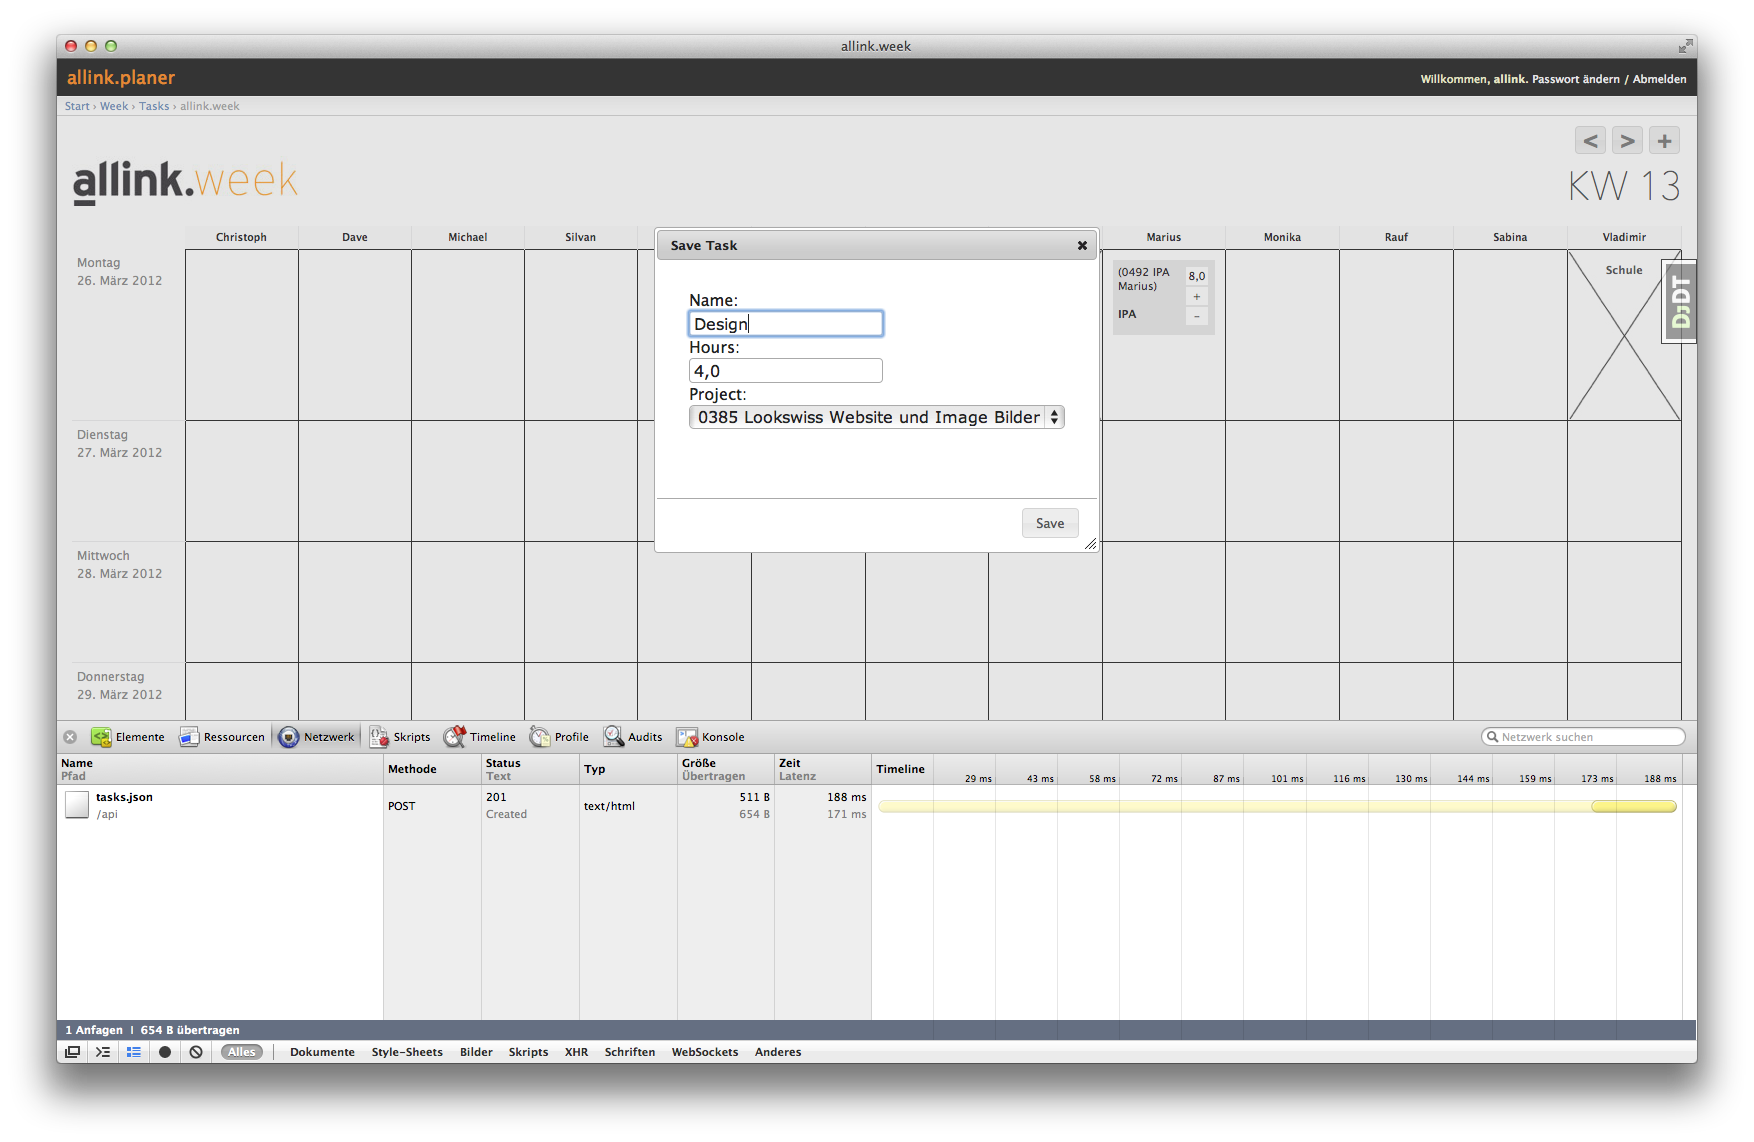
\includegraphics[width=0.99\textwidth,angle=0]{bilder/testing/Task_erstellen.png}
    \caption{Nr. 1, 2, 3, 4, 5, 12}
    \label{fig:bilder_testing_Task erstellen}
\end{figure}
\begin{figure}[htbp]
    \centering
        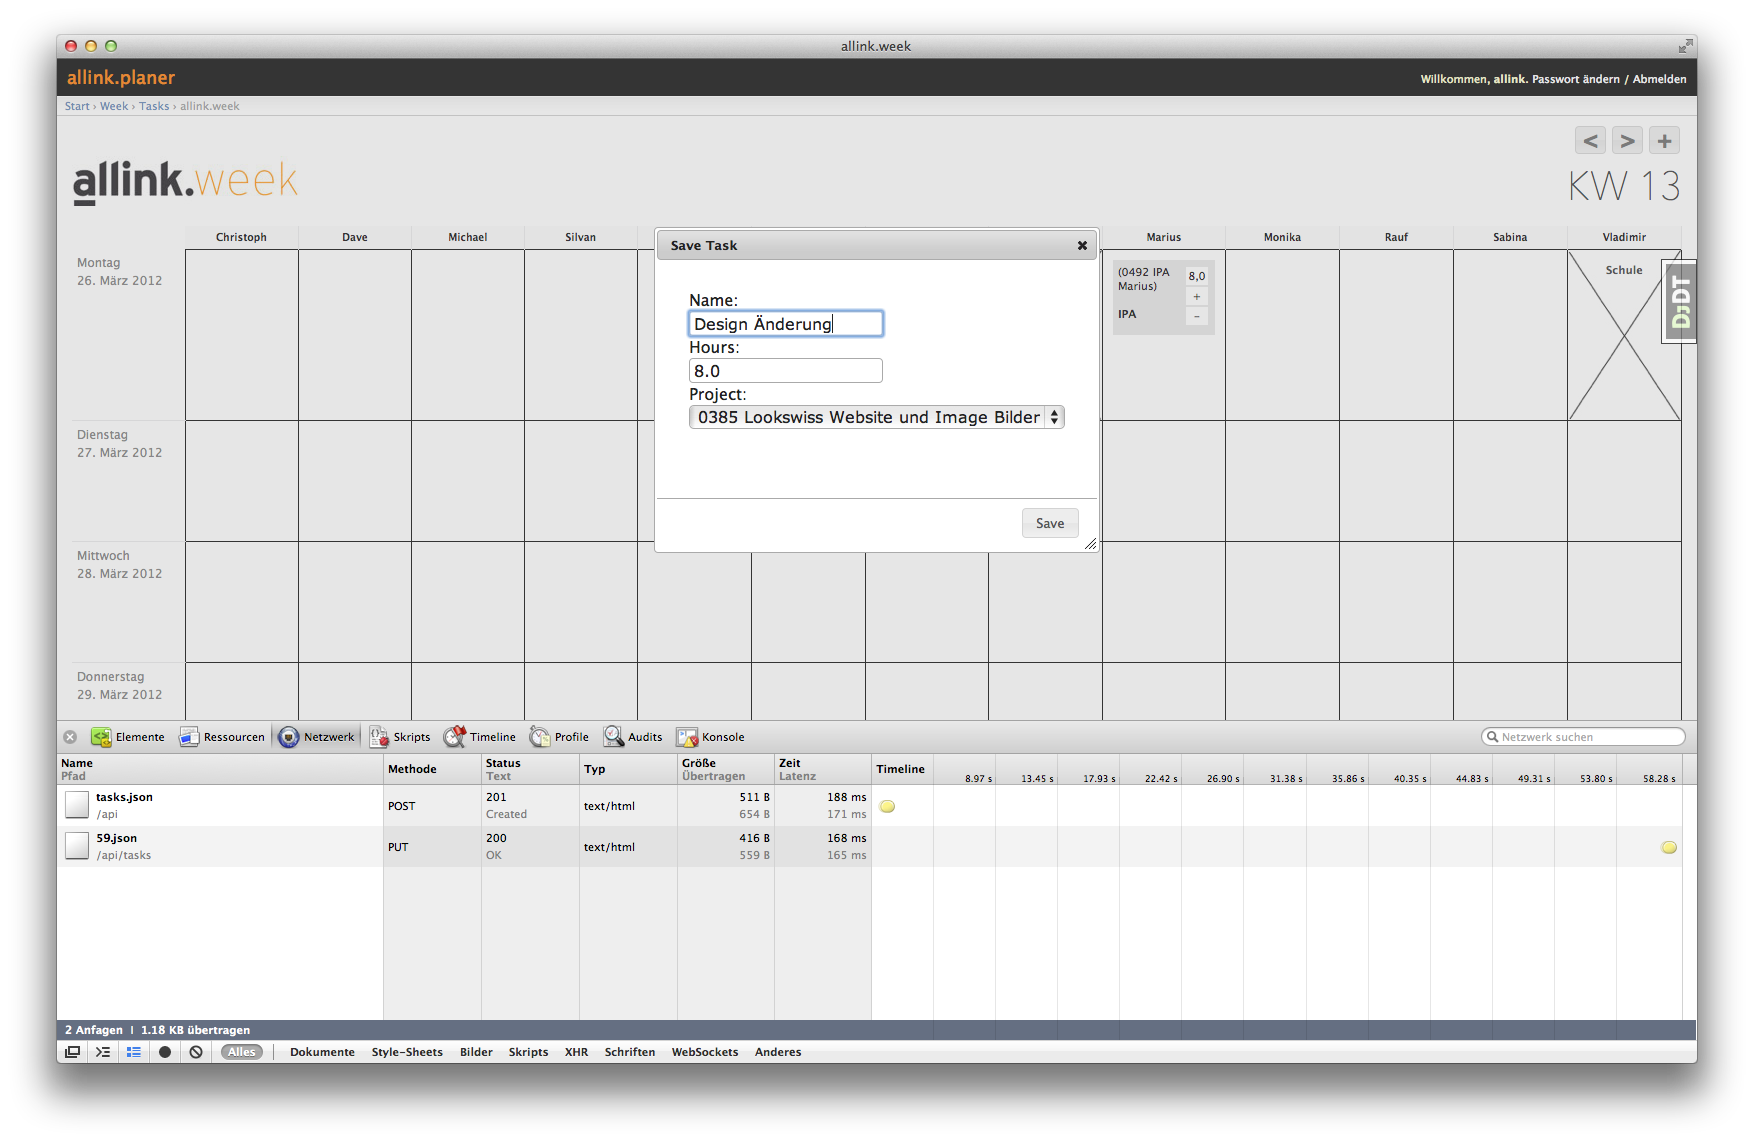
\includegraphics[width=0.99\textwidth,angle=0]{bilder/testing/Task_bearbeiten.png}
    \caption{Nr. 6}
    \label{fig:bilder_testing_Task_bearbeiten}
\end{figure}
\begin{figure}[htbp]
    \centering
        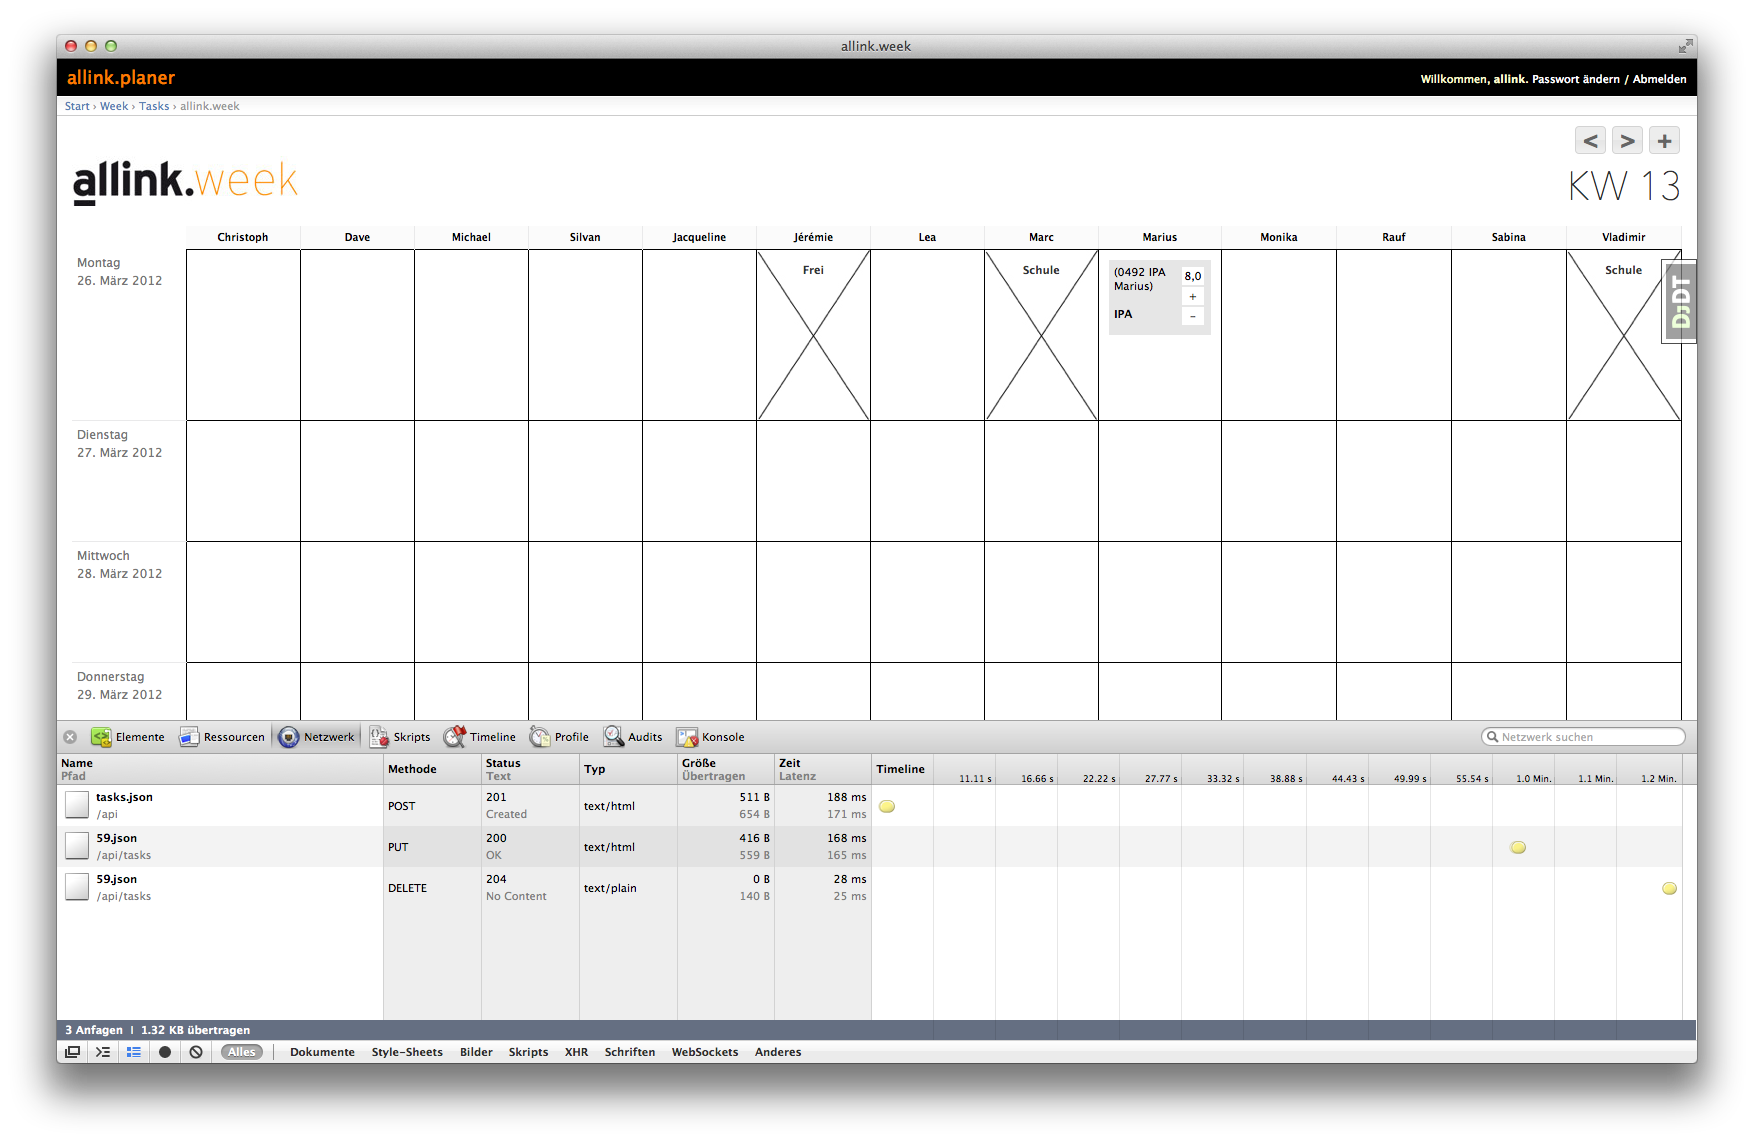
\includegraphics[width=0.99\textwidth,angle=0]{bilder/testing/Task_loeschen.png}
    \caption{Nr. 7}
    \label{fig:bilder_testing_Task_loeschen}
\end{figure}
\begin{figure}[htbp]
    \centering
        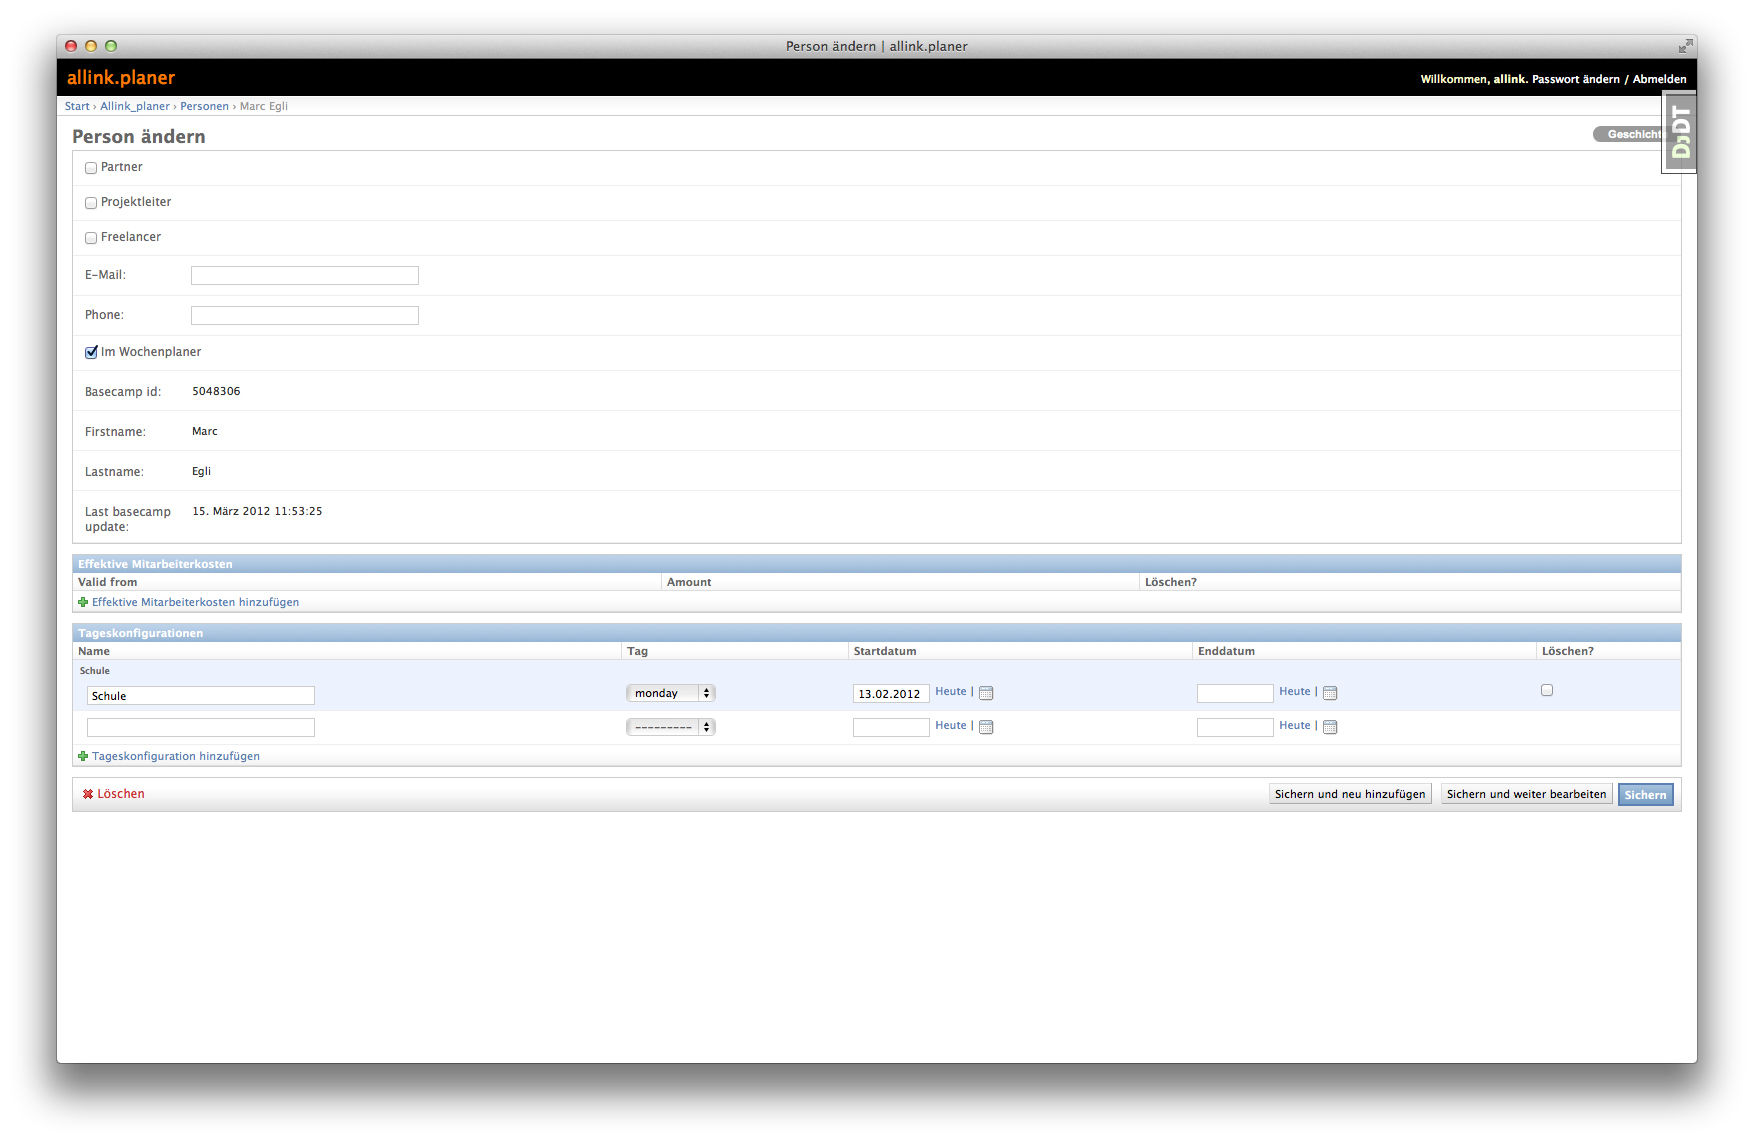
\includegraphics[width=0.99\textwidth,angle=0]{bilder/testing/Sperrtag_erstellen.png}
    \caption{Nr. 8, 9}
    \label{fig:bilder_testing_Sperrtag_erstellen}
\end{figure}
\begin{figure}[htbp]
    \centering
        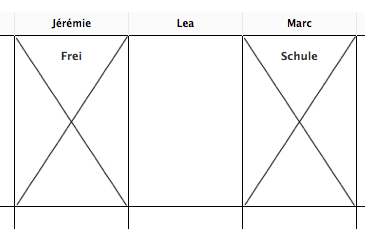
\includegraphics[width=0.99\textwidth,angle=0]{bilder/testing/Sperrtag_Person_zuweisen.png}
    \caption{Nr. 8, 9}
    \label{fig:bilder_testing_Sperrtag_Person_zuweisen}
\end{figure}
\begin{figure}[htbp]
    \centering
        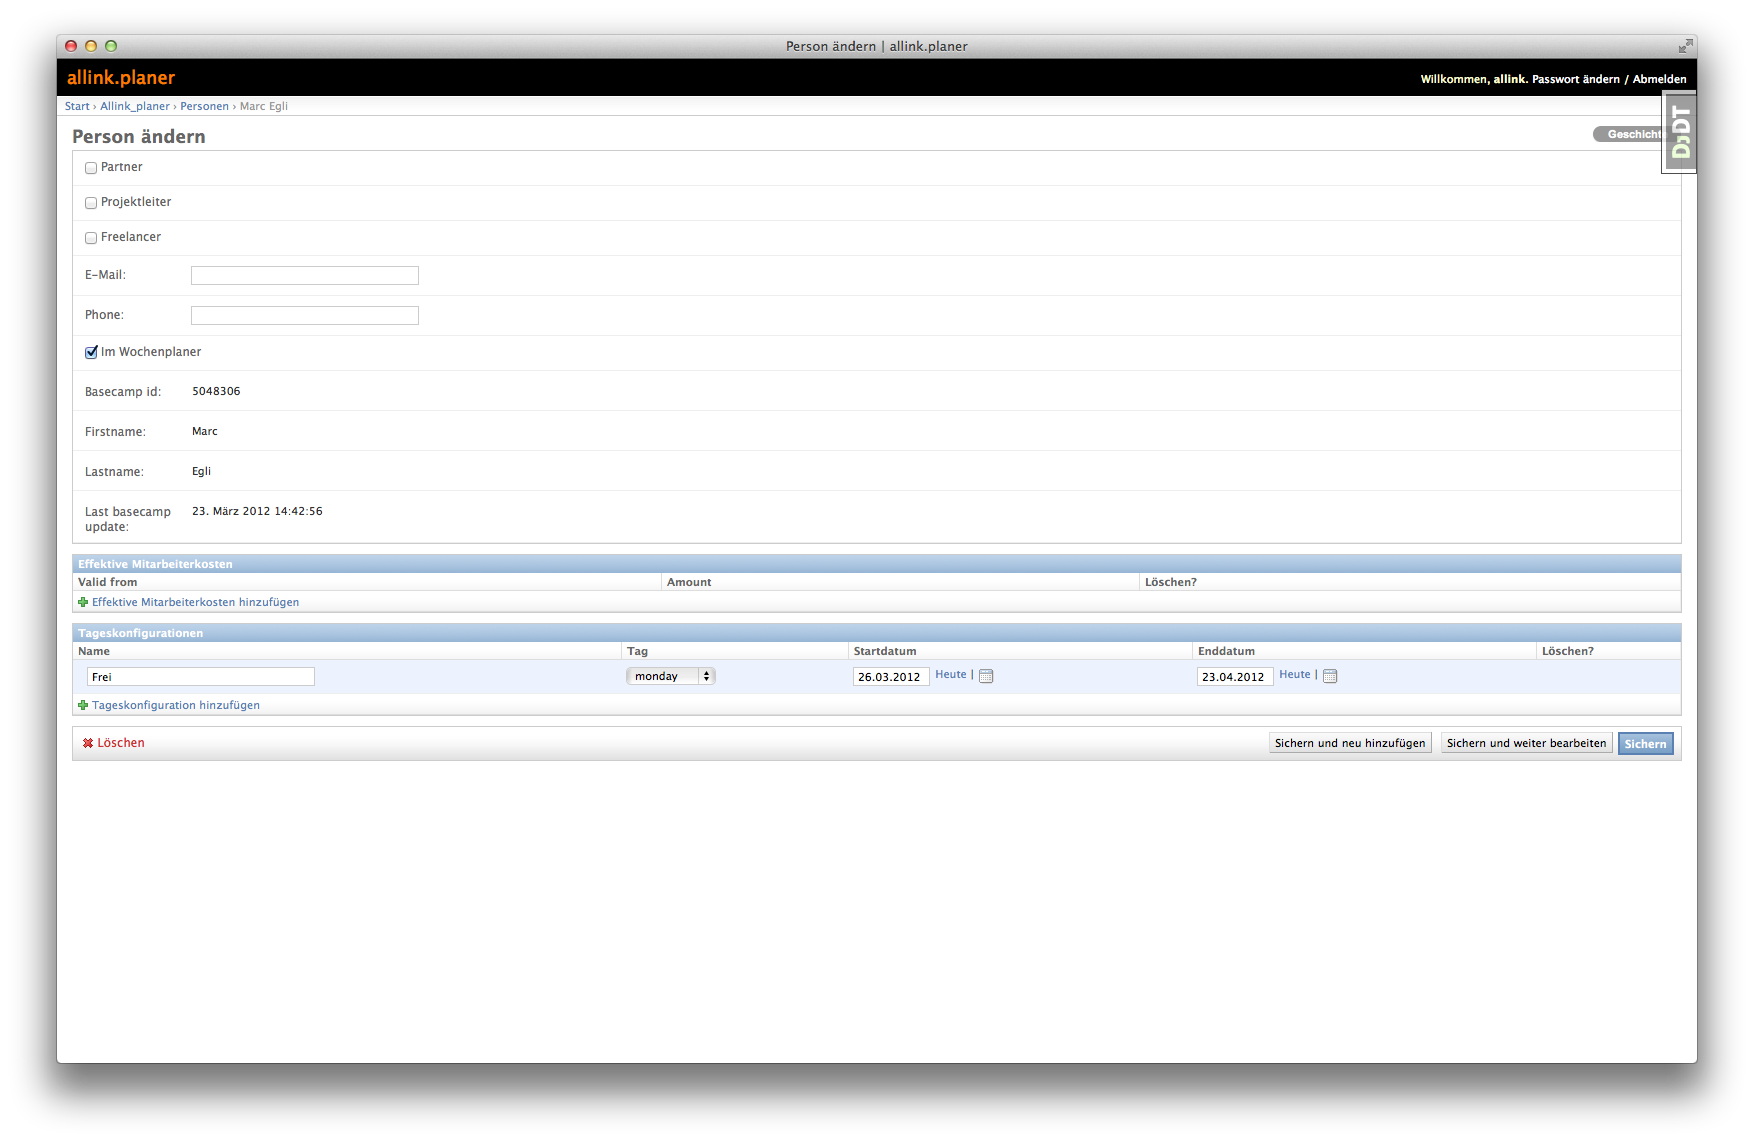
\includegraphics[width=0.99\textwidth,angle=0]{bilder/testing/Sperrtag_bearbeiten.png}
    \caption{Nr. 10}
    \label{fig:bilder_testing_Sperrtag_bearbeiten}
\end{figure}
\begin{figure}[htbp]
    \centering
        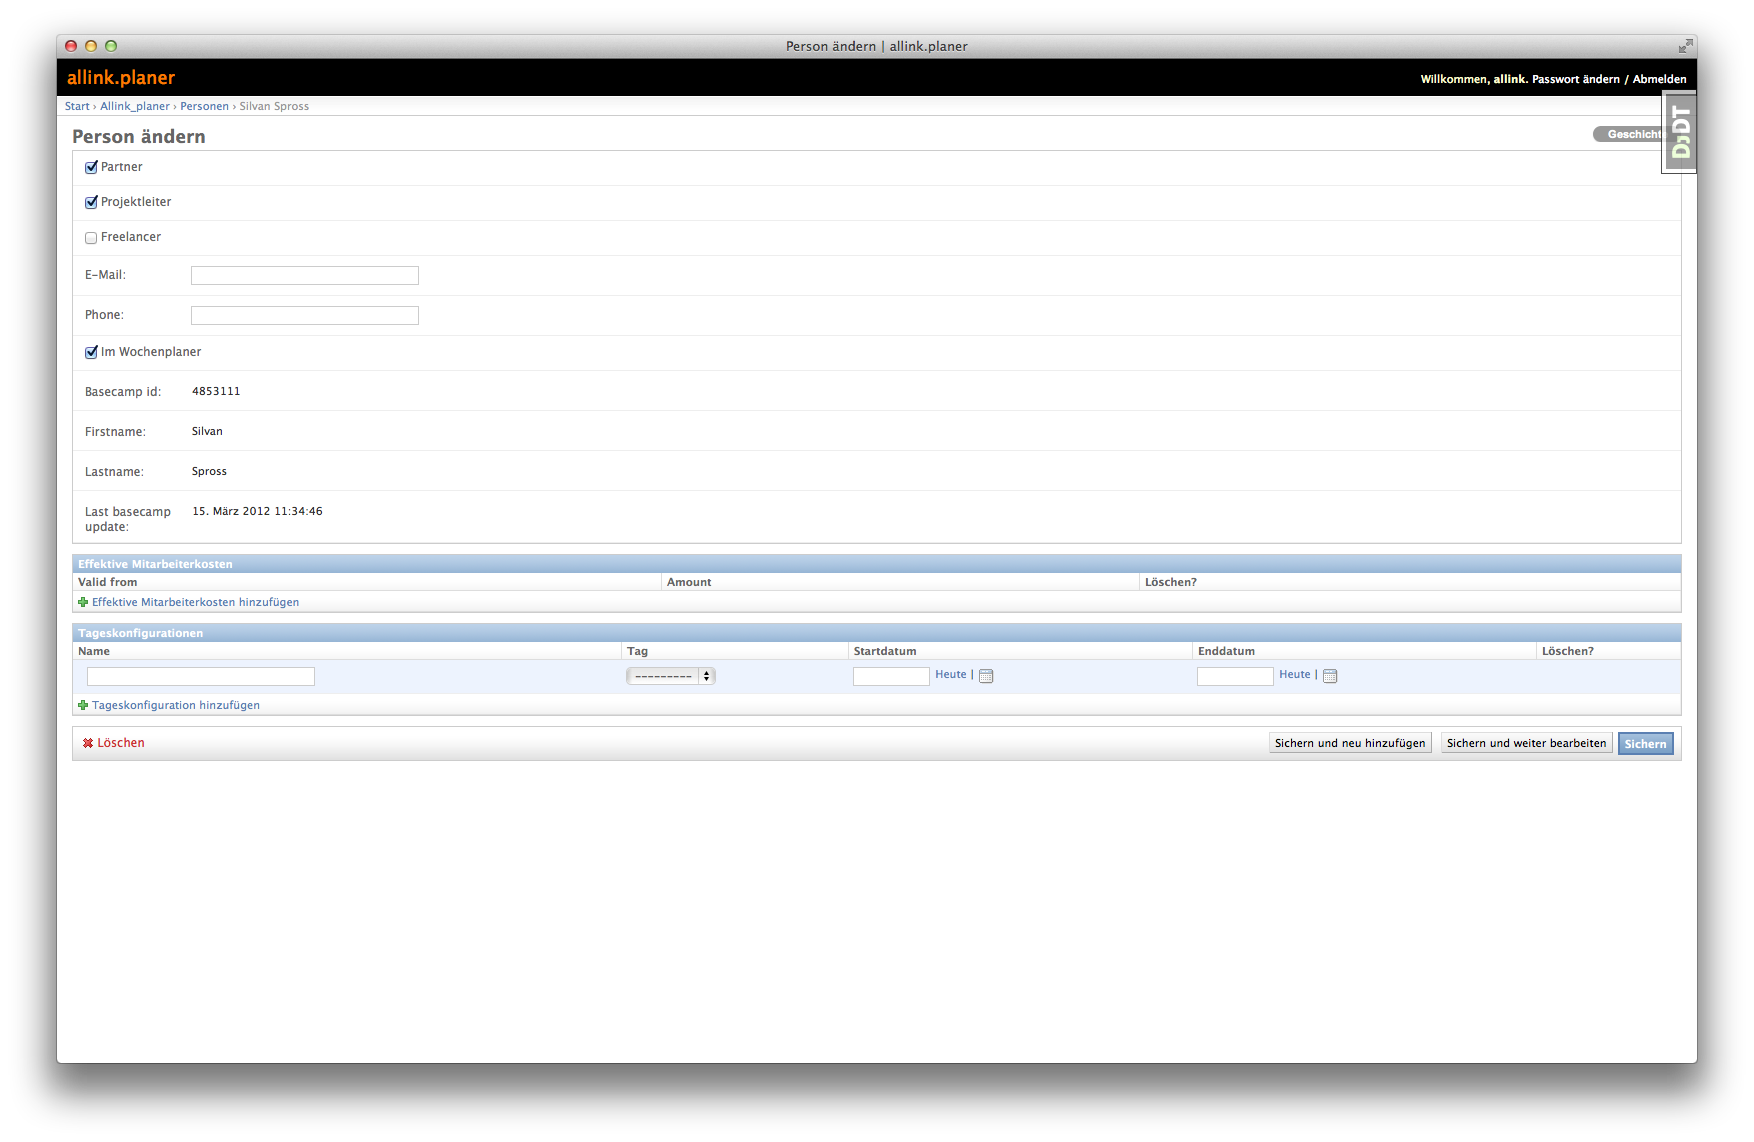
\includegraphics[width=0.99\textwidth,angle=0]{bilder/testing/Sperrtag_loeschen.png}
    \caption{Nr. 11}
    \label{fig:bilder_testing_Sperrtag_loeschen}
\end{figure}
\begin{figure}[htbp]
    \centering
        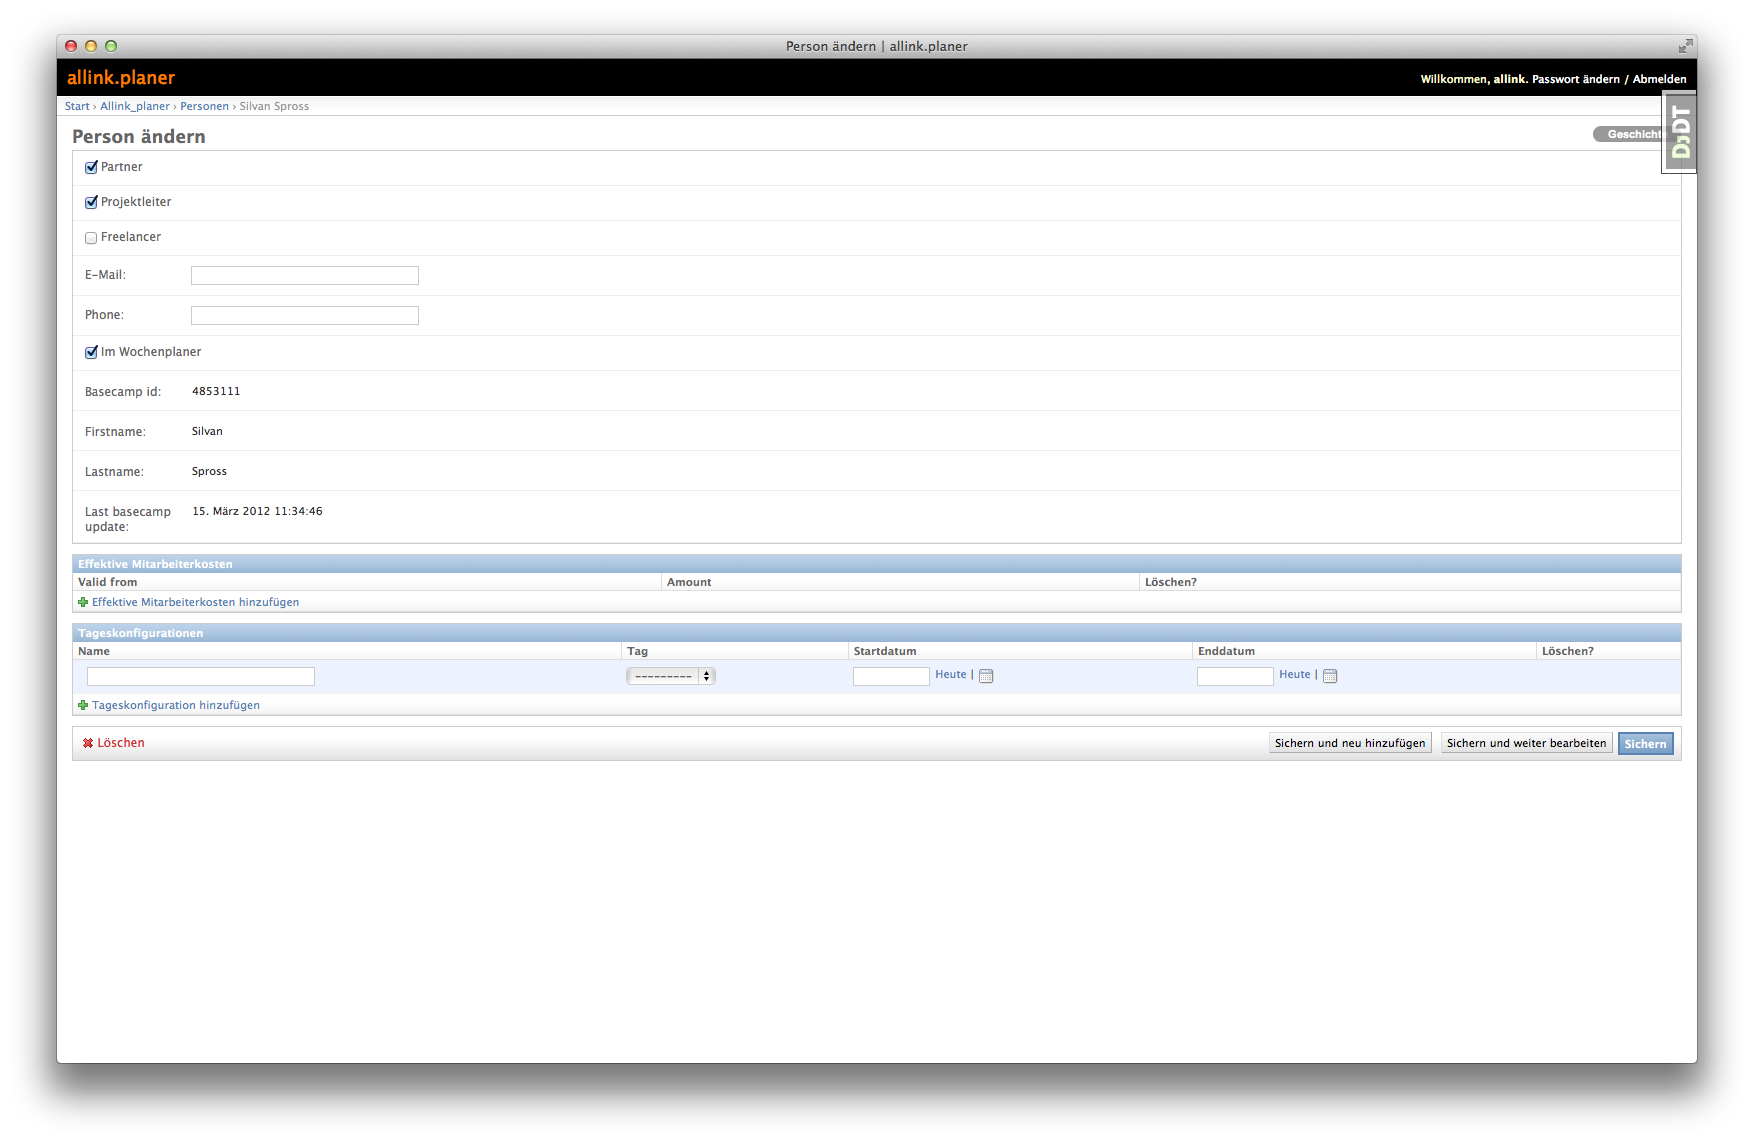
\includegraphics[width=0.99\textwidth,angle=0]{bilder/testing/Person_wochenplaner_partner.png}
    \caption{Nr. 13, 14}
    \label{fig:bilder_testing_Person_wochenplaner_partner}
\end{figure}
\begin{figure}[htbp]
    \centering
        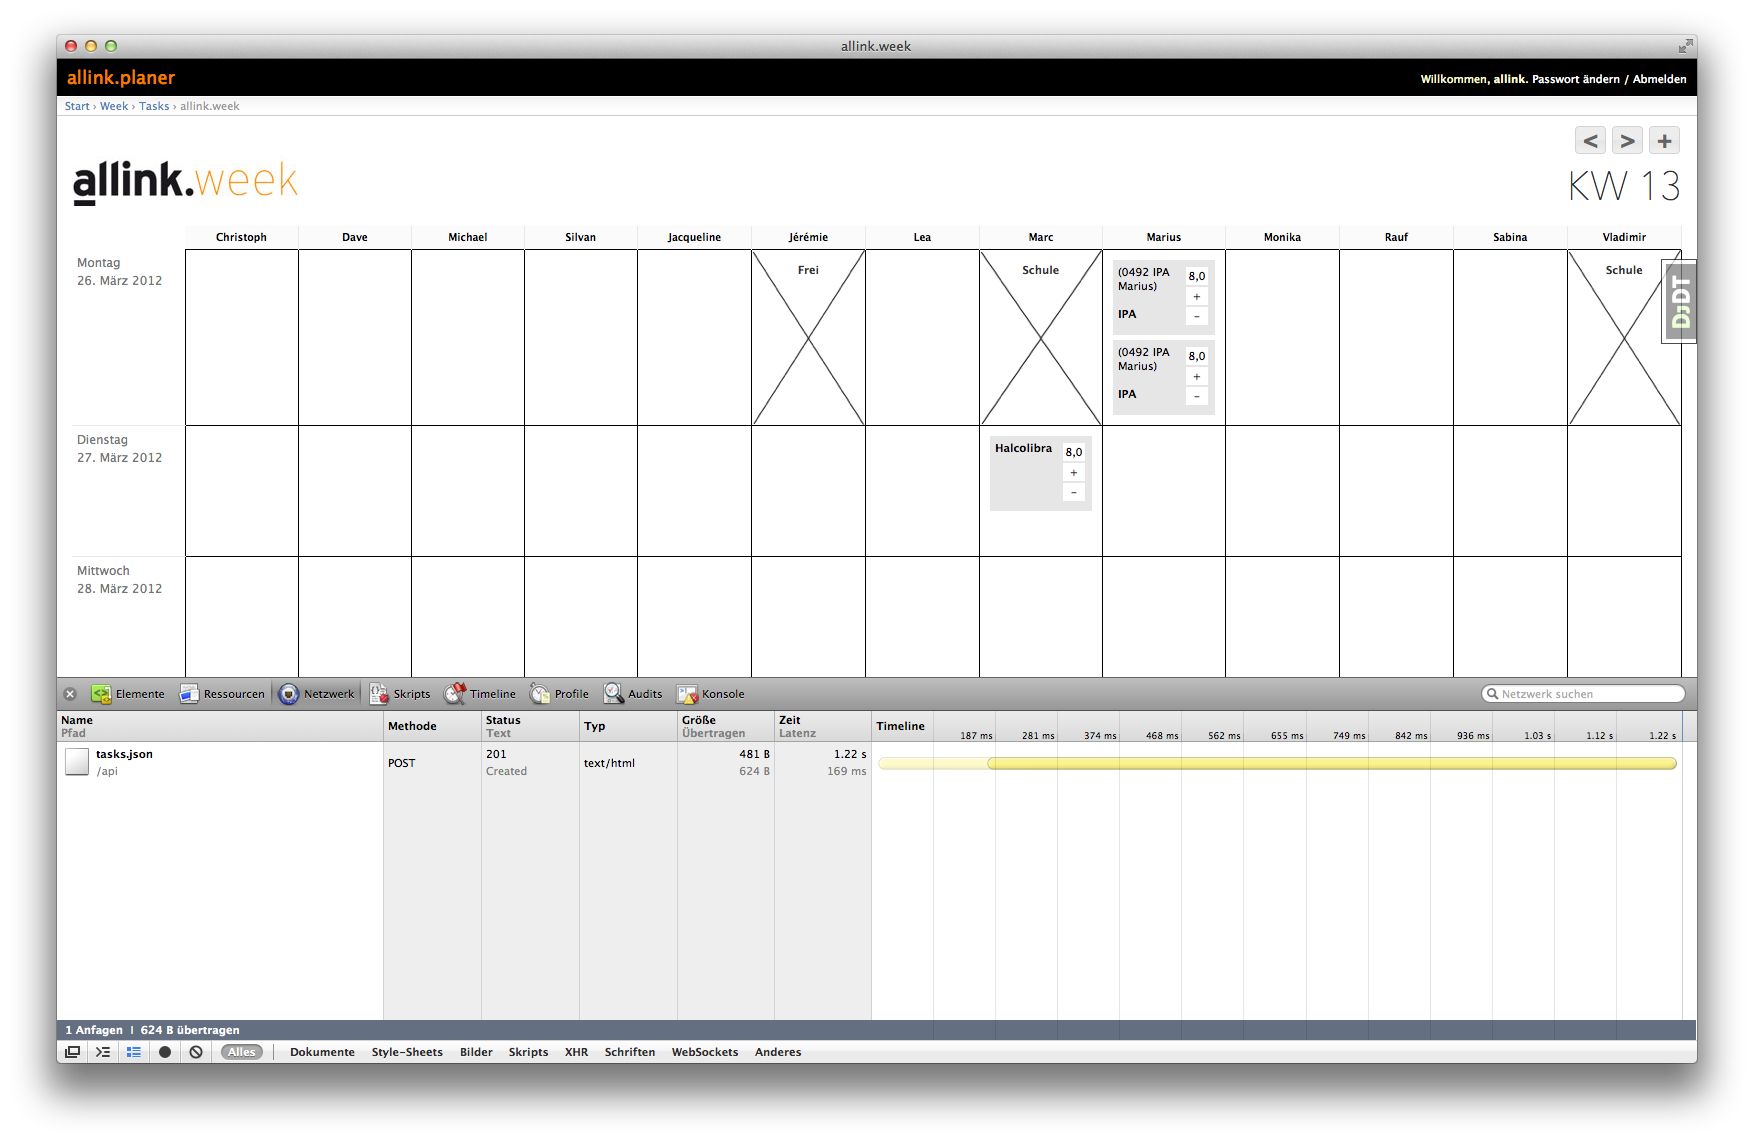
\includegraphics[width=0.99\textwidth,angle=0]{bilder/testing/Task_duplizieren.png}
    \caption{Nr. 15}
    \label{fig:bilder_testing_Task_duplizieren}
\end{figure}
\begin{figure}[htbp]
    \centering
        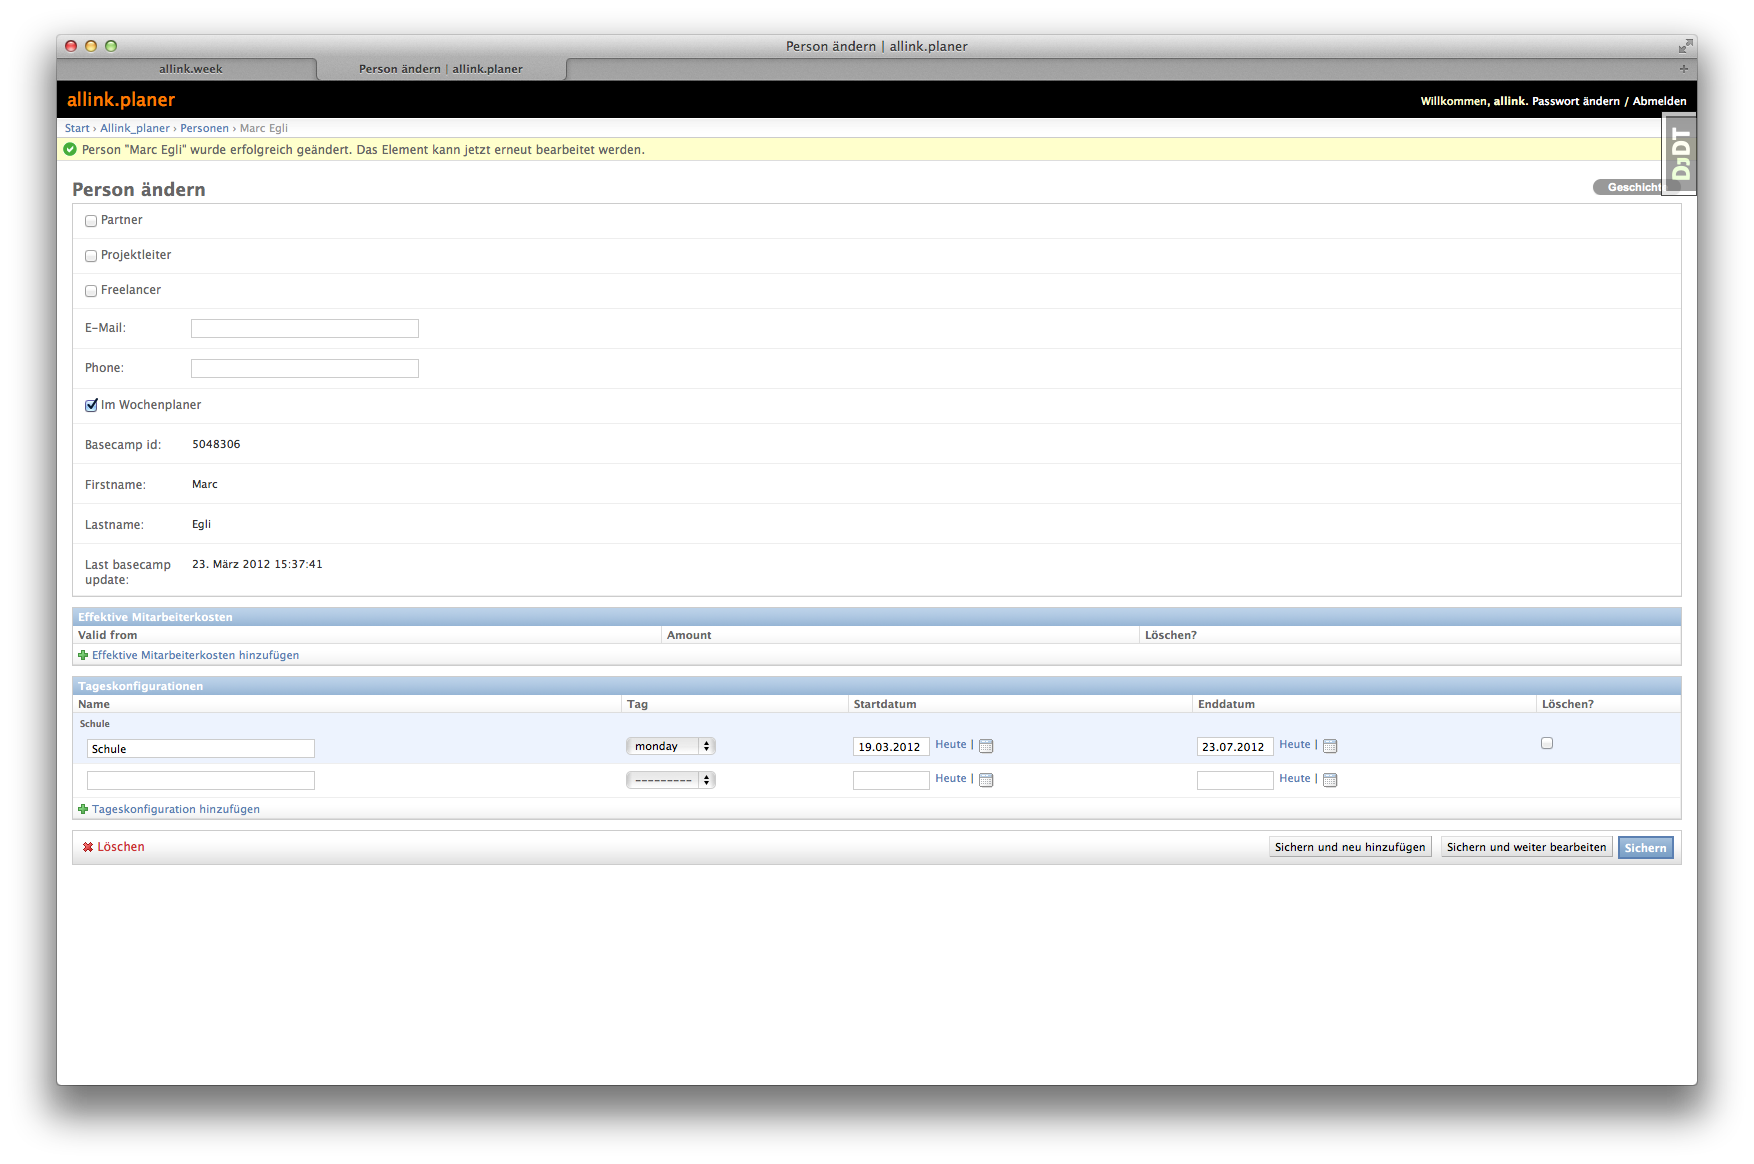
\includegraphics[width=0.99\textwidth,angle=0]{bilder/testing/Sperrtag_start_end.png}
    \caption{Nr. 16}
    \label{fig:bilder_testing_Sperrtag_start_end}
\end{figure}
\begin{figure}[htbp]
    \centering
        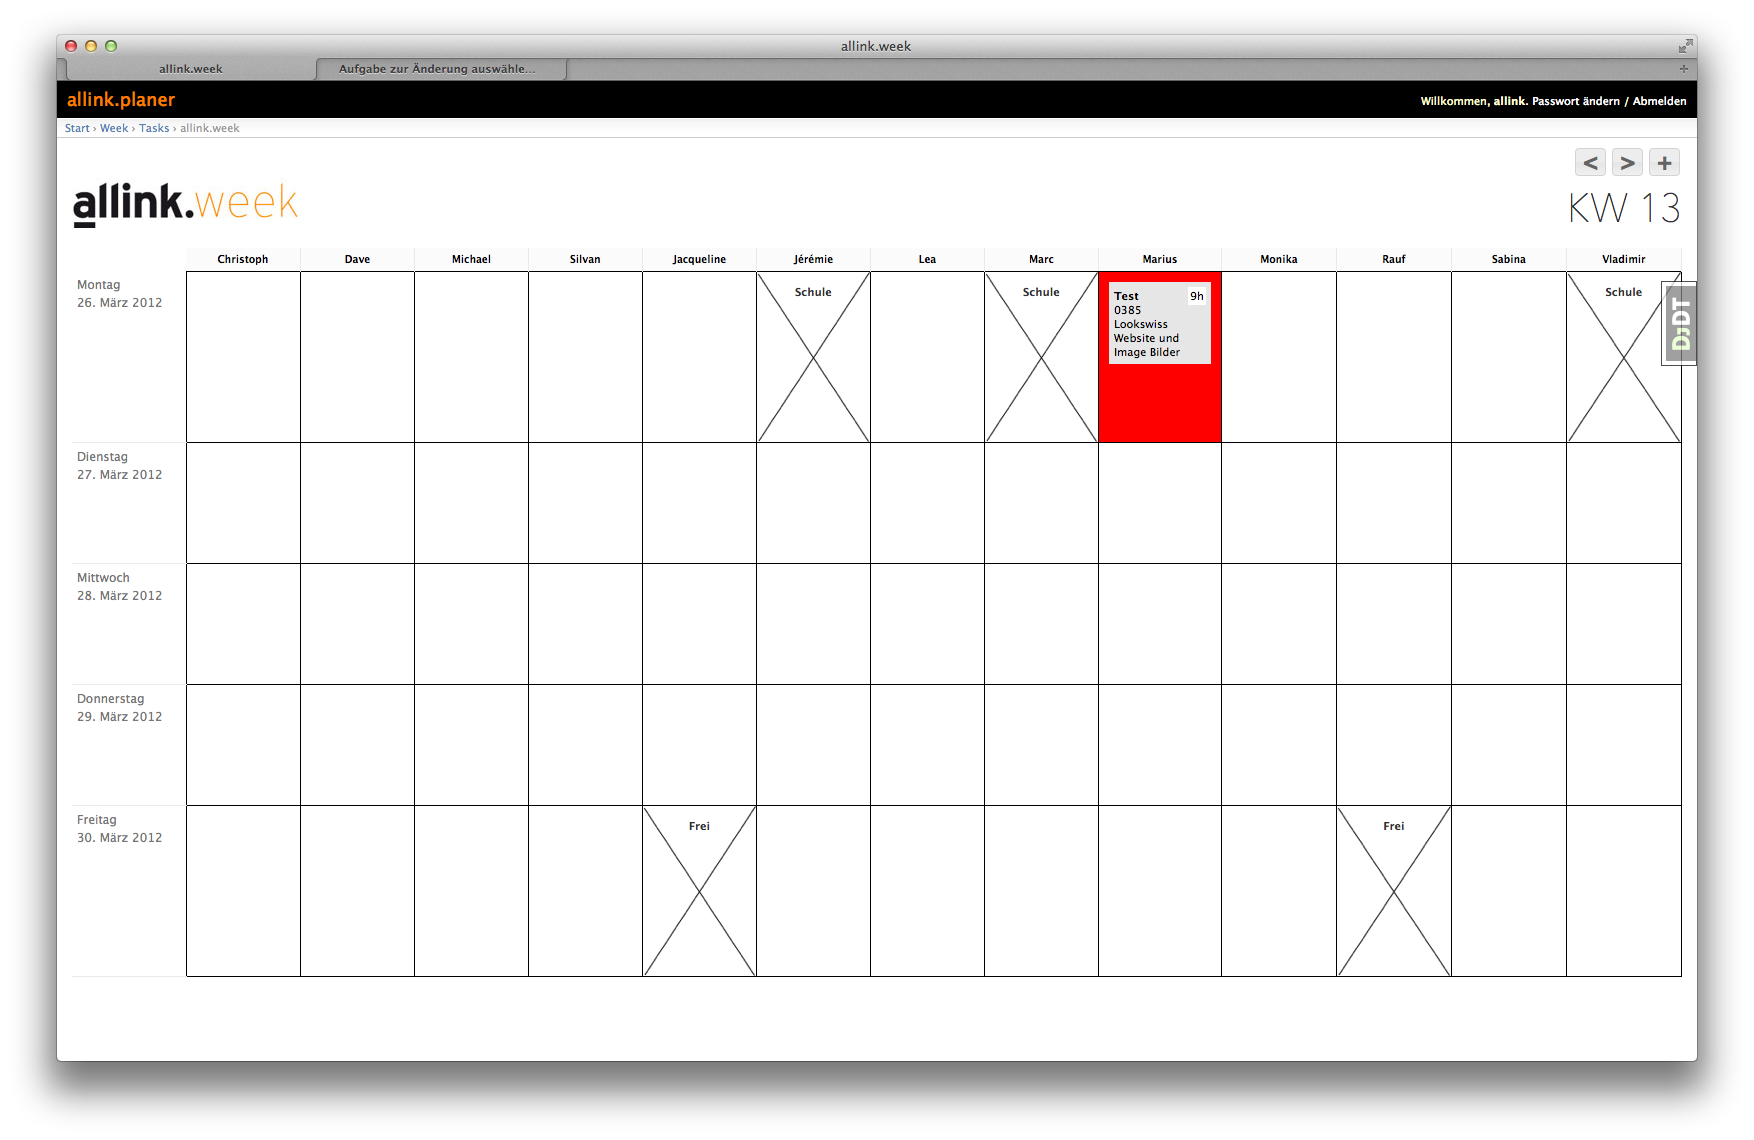
\includegraphics[width=0.99\textwidth,angle=0]{bilder/testing/warnmeldung.png}
    \caption{Nr. 17}
    \label{fig:bilder_testing_warnmeldung}
\end{figure}
\begin{figure}[htbp]
    \centering
        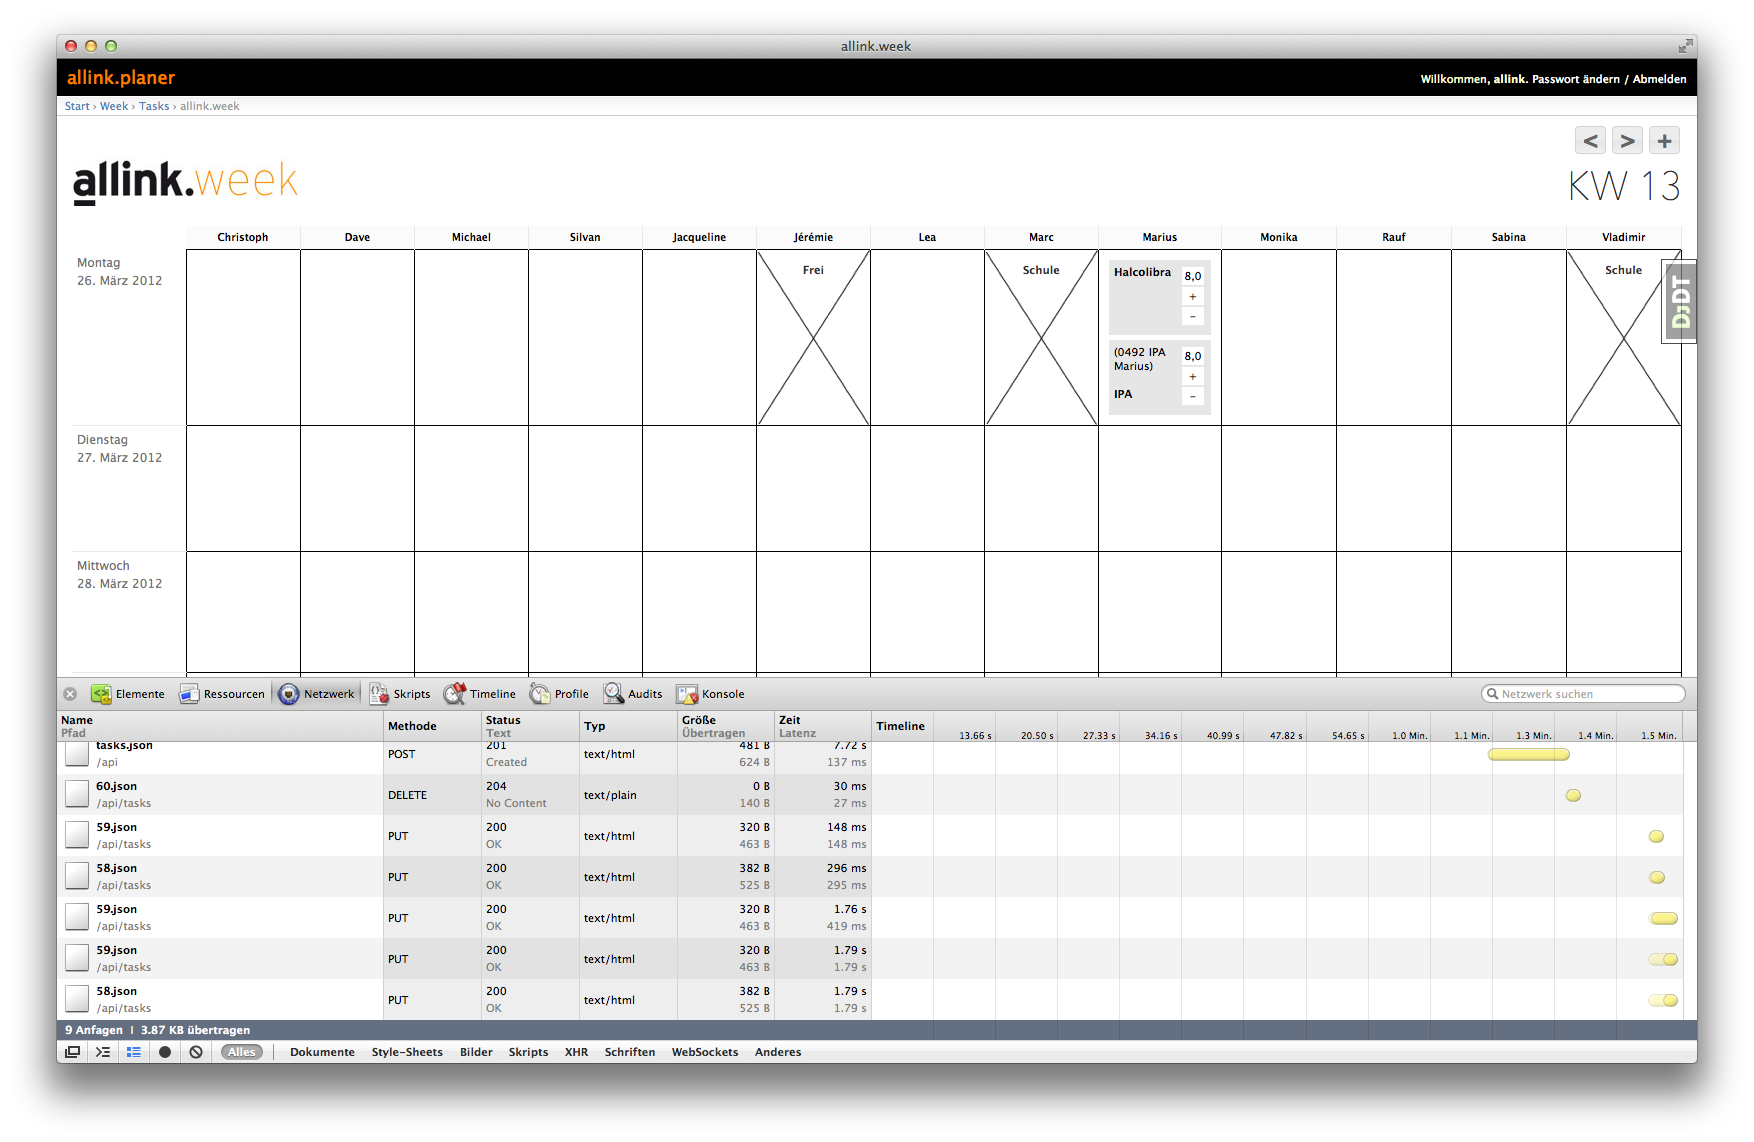
\includegraphics[width=0.99\textwidth,angle=0]{bilder/testing/tasks_sortieren.png}
    \caption{Nr. 18}
    \label{fig:bilder_testing_tasks_sortieren}
\end{figure}
\clearpage
\subsection{Erfolge Testing}
Hier liste ich alle Tests auf und zeige ob sie erfolgreich waren oder nicht.
\begin{table}[!ht]
\begin{center}
    \begin{tabular}{llp{8cm}l}
        \toprule Nr & MUSS-Funktion & erfolgreich? \\
        \midrule 1 & 1 & ja\\
        \midrule 2 & 2 & ja\\
        \midrule 3 & 3 & ja\\
        \midrule 4 & 4 & ja\\
        \midrule 5 & 5 & ja\\
        \midrule 6 & 6 & ja\\
        \midrule 7 & 7 & ja\\
        \midrule 8 & 8 & ja\\
        \midrule 9 & 9 & ja\\
        \midrule 10 & 10 & ja\\
        \midrule 11 & 11 & ja\\
        \midrule 12 & 12 & ja\\
        \midrule 13 & 13 & ja\\
        \midrule 14 & 14 & ja\\
        \midrule 15 & 15 & ja\\
        \midrule 16 & 16 & ja\\
        \midrule 17 & 17 & ja\\
        \midrule 18 & 18 & ja\\
        \bottomrule
    \end{tabular}
    \caption{Zu erfüllende Funktionen des Prototypen}
    \label{tab:testing_muss_funktionen_ziele}
\end{center}
\end{table}
\footnotetext{Eigene Darstellung}
\subsection{Field-Test}
Am 24.03. wird die Geschäftsführung an ihrer wöchentlichen Planungssitzung das Tool das erste Mal verwenden.
Dabei soll das Tool auf sein Intuitivität geprüft werden. Am Montag werde ich dann Feedback erhalten und anfallende Anpassungen vornehmen.
